
\section{Command-V in Practice}
\label{sec-experiments}
We port three behaviors chosen for large pre/post-finetuning gaps, easy verification, and practical utility: refusal enhancement, refusal suppression (jailbreak), and default chain-of-thought.

\paragraph{Adapter training.}
DiReFT on every other donor layer, last-token only, rank 8, 6 epochs, batch sizes 2 / 4 / 16 following Wu et al.~\cite{wu2024reft} Table~6 with those exceptions.

\subsection{Case study: refusal enhancement}

We train on 10,000 WildJailbreak~\cite{jiang2024} training prompts (harmful and benign adversarial).
Evaluation uses all 2,000 adversarial harmful and 221 adversarial benign prompts from the evaluation split.
LlamaGuard3 8B~\cite{grattafiori2024} labels harmful responses; we manually inspect benign overrefusal.

\obtodo[id=cv-refusal-train, created=2025-04-02T09:00:00.000Z, updated=2025-04-18T23:41:10.000Z, completed=2025-04-18T23:41:10.000Z]{Train DiReFT refusal adapters on Llama-3.1-8B and Llama-3.2-3B, WildJailbreak 10k, conservative batch 2/4.}
\obtodo[id=cv-refusal-eval, created=2025-04-19T10:15:00.000Z, updated=2025-04-27T14:08:33.000Z, completed=2025-04-27T14:08:33.000Z]{Plot ASR vs A100-40GB wall time for ReFT checkpoints and Command-V, including amortized profiling cost.}

A completed 3B adapter drops test ASR from $31.30\%$ to $12.20\%$ (intermediary low $5.65\%$).
Ported onto 8B, ASR falls $36.85\%\to 20.40\%$, beating direct 8B ReFT ($28.55\%$, intermediary low $21.05\%$).
The reverse 8B$\to$3B paste reaches $16.4\%$ ASR (Figure~\ref{fig:refusal}).

\begin{figure}[t]
\centering
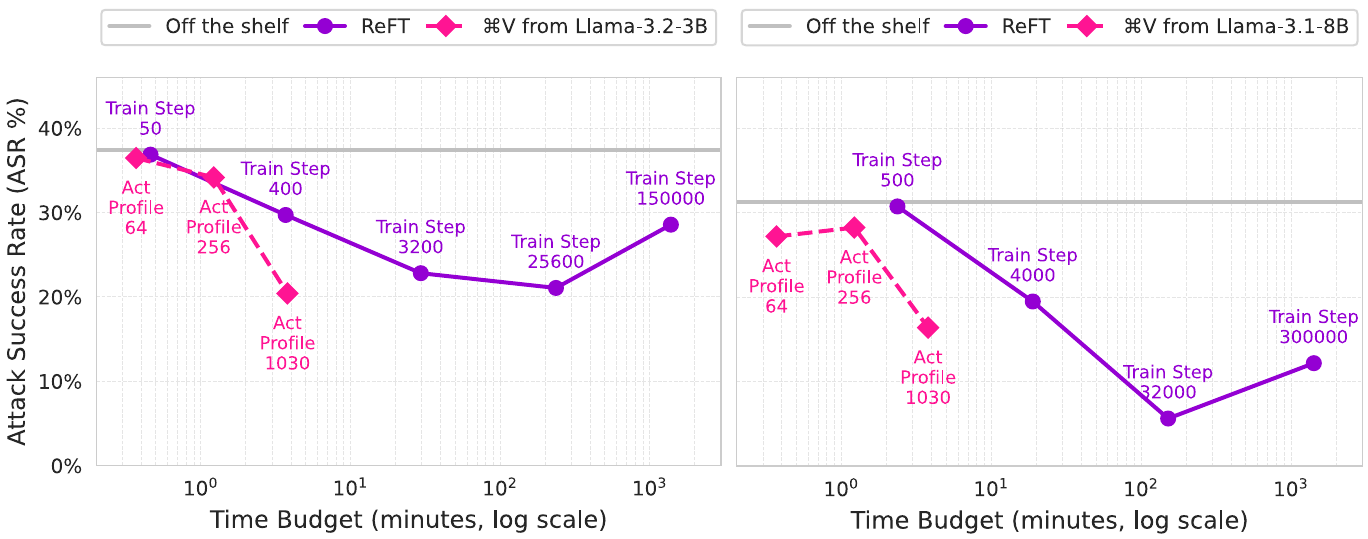
\includegraphics[width=\linewidth]{figures/WildJailbreak.png}
\caption{Reduced jailbreak attack success rate (ASR $\downarrow$) on Llama-3.2-3B-Instruct (left) and Llama-3.1-8B-Instruct (right).
Purple: WildJailbreak ReFT. Pink: \cmdv{}.
\cmdv{} sits on the cost--performance Pareto frontier. Time is A100 40GB wall time.}
\label{fig:refusal}
\end{figure}

\obcomment[kind=result]{3B adapter pasted onto 8B beats training the 8B adapter directly (20.40 vs 28.55 ASR). Keep that as the teaser number. Larger ReFT batches (12/16) trained faster and defended worse --- do not quote those.}

\paragraph{Overrefusal.}
Undesirable refusals on jailbreak-shaped but legitimate queries increase with ReFT and more with \cmdv{} (Table~\ref{tab:overrefusal}).

\begin{table}[t]
\centering
\caption{Human-annotated overrefusal rate ($\downarrow$) on WildJailbreak adversarial-benign test prompts.}
\label{tab:overrefusal}
\begin{tabular}{lccc}
\toprule
Model & Off-shelf (\%) & ReFT (\%) & \cmdv{} (\%) \\
\midrule
Llama 3.1 8B & 1.36 & 2.26 & 4.52 \\
Llama 3.2 3B & 3.17 & 8.60 & 14.48 \\
\bottomrule
\end{tabular}
\end{table}

\obtodo[id=cv-overrefusal, created=2025-04-28T13:00:00.000Z, updated=2025-05-06T19:22:47.000Z, completed=2025-05-06T19:22:47.000Z]{Human-label overrefusal on the 221 adversarial-benign prompts for off-shelf, ReFT, and Command-V.}

\paragraph{Efficiency.}
Profiling is a forward pass, amortized per model.
Converters take 6.35s mean on a MacBook Pro CPU for 14--18 layer pairs.

\subsection{Case study: refusal suppression}

Train and evaluate on AdvBench~\cite{zou2023advbench}; transfer-check on HarmBench Standard~\cite{mazeika2024}.
LlamaGuard3 8B is the safety classifier.
We port across Llama~3, Qwen2.5, and Gemma~2 instruct models, and additionally run inference-only recipients Phi-4-mini and OLMo~2 (not trainable in the ReFT library at the time).

\obtodo[id=cv-jailbreak-matrix, created=2025-05-07T09:30:00.000Z, updated=2025-05-28T02:17:09.000Z, completed=2025-05-28T02:17:09.000Z]{Fill the AdvBench and HarmBench donor-recipient ASR heatmaps, including same-family boxes.}

\begin{figure}[hpt]
\centering
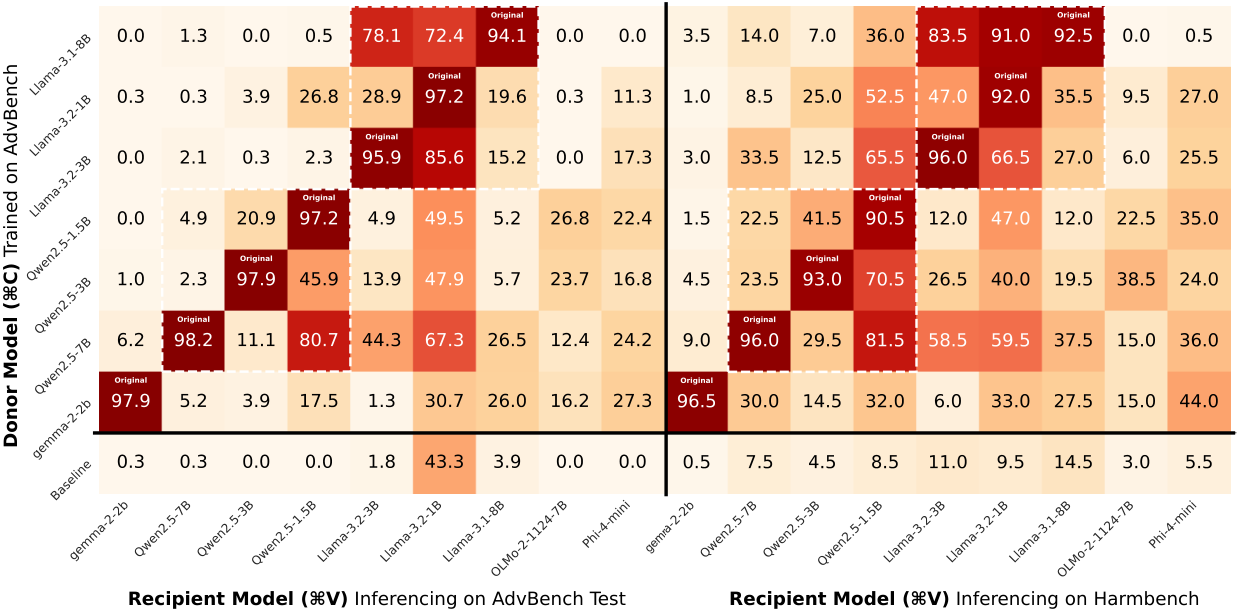
\includegraphics[width=0.99\linewidth]{figures/grid.png}
\caption{Jailbreaking and \cmdv{}: porting jailbreakability often increases ASR ($\uparrow$), especially in the same model family (white dashed boxes).
Diagonal entries are ReFT adapter validation performance, an upper bound on expected \cmdv{} transfer.
All models are instruct versions.}
\label{fig:grid}
\end{figure}

Off-shelf models sit at single-digit ASR (Figure~\ref{fig:grid}).
After \cmdv{}, many jump to $20$--$80\%$.
Qwen2.5-7B-Instruct is the best donor: mean $41.2\%$ AdvBench and $46.9\%$ HarmBench when ported, up to $80.7\%$ / $81.5\%$ on Qwen2.5-1.5B-Instruct.
Llama-3.2-1B-Instruct is the most susceptible recipient (mean $61.7\%$ / $54.9\%$).
Gemma2-2B-it is the most resistant: no donor jailbreaks it meaningfully.
Same-family transfers dominate the heatmaps.
LIMA profiles were not collected on harmful prompts and still transferred.

\obcomment[kind=result]{Qwen2.5-7B donor is the jailbreak workhorse. Gemma2-2B-it refused every paste. Put both in the caption so the heatmap is not read as universal transfer.}

\subsection{Case study: increased use of chain-of-thought}

We train ReFT on 2,000 OpenMathReasoning~\cite{moshkov2025} examples, replacing specialized thinking delimiter tokens with natural words to avoid tokenizer-mismatch garbage after porting.
Evaluation: two Big-Bench Hard~\cite{suzgun2022} tasks with the largest original CoT lifts, 250 test questions each, answers requested as short JSON.

\obtodo[id=cv-cot-openmath, created=2025-05-12T10:00:00.000Z, updated=2025-06-09T18:51:26.000Z, completed=2025-06-09T18:51:26.000Z]{Port OpenMathReasoning CoT adapters across Qwen2.5 and Llama 3.1/3.2 sizes on BBH multistep arithmetic and tracking shuffled objects.}

\begin{figure}[h]
\centering
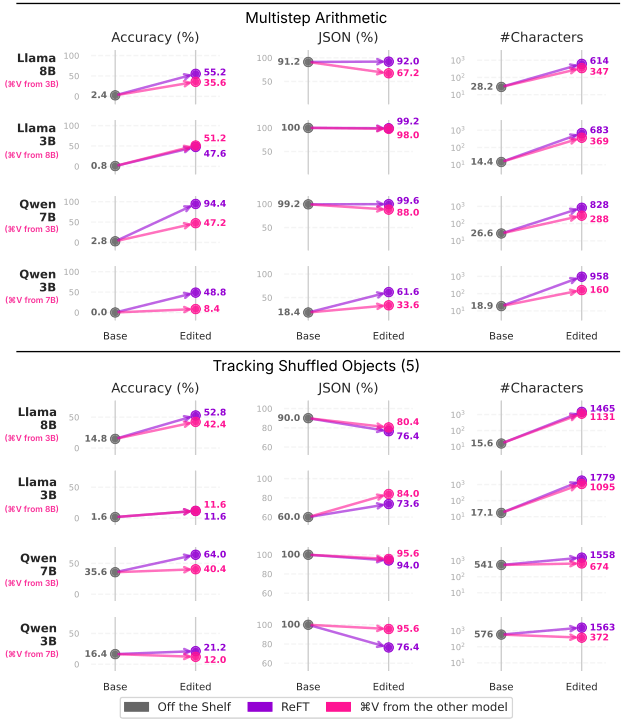
\includegraphics[width=0.85\linewidth]{figures/reasoning2.png}
\caption{Trained and \cmdv{} performance on Big-Bench Hard.
Same-family OpenMathReasoning ports increase output length and task accuracy, comparable to direct ReFT, while more responses fail the requested JSON format (middle column).}
\label{fig:cot}
\end{figure}

JSON makes extraction easy and depresses absolute accuracy relative to unconstrained decoding (Figure~\ref{fig:cot}).
Multistep arithmetic sees marked gains; Qwen2.5-3B is the largest porting lift ($+50\%$).
Tracking shuffled objects is a smaller but real lift, especially on larger models.
Reasoning quality improved uniformly; instruction following sometimes collapsed, with up to $28.8\%$ of responses failing the JSON format, plus occasional language drift on Qwen.

\obcomment[kind=result]{CoT paste works as more characters and higher task accuracy, with a format-collapse tax. Do not bury the 28.8 percent JSON failure --- it is the honest limitation next to the +50 percent Qwen 3B lift.}
